\documentclass[12pt]{article}
\usepackage[T1]{fontenc}
\usepackage{enumitem}
\usepackage[english]{babel}
\usepackage{graphicx,epstopdf,url}
\usepackage{float}
\usepackage{amsmath}

\usepackage[top=0.8in, bottom=1in, left=1in, right=1in]{geometry}

\title{NCA - Lab report \\

Random number generation
}
\author{\bf{Group 10} \\ \\
        Abdul Hadi Farooq \\
        Ali Haider \\
        Ali Raza \\
}

\date{April 12, 2026}

\begin{document}

\maketitle

\section{Introduction}

The objective of this laboratory is to understand the behavior and properties of random variable distributions through computational generation and visualization. Random number generation is fundamental to performance evaluation, simulation studies, and statistical modeling of computer systems.

In this work, we generate five different probability distributions with varying sample sizes to observe how the empirical distribution converges to the theoretical distribution as the number of samples increases. The distributions studied are: Uniform (Integer), Uniform (Double), Normal, Exponential, and Lognormal.

All random number generation was performed using the NumPy library with a fixed seed value of 10 to ensure reproducibility. For each distribution, we generated samples of sizes $n \in \{10, 100, 1000, 10000\}$ to observe convergence behavior. The histograms visualize the empirical frequency distributions and demonstrate how the Law of Large Numbers applies to each distribution type.

\subsection{Methodology}

\begin{itemize}
    \item \textbf{Programming Language:} Python with NumPy and Matplotlib
    \item \textbf{Random Seed:} 10 (ensures reproducibility---same seed always produces identical sequences)
    \item \textbf{Sample Sizes:} $n = 10, 100, 1000, 10000$
    \item \textbf{Total Test Cases:} 20 (5 distributions $\times$ 4 sample sizes)
    \item \textbf{Histogram Binning:} Sturges rule (automatic bin calculation based on sample size)
    \item \textbf{Reproducibility:} All results verified by re-running with identical seed---identical outputs confirmed
\end{itemize}

\subsection{Code Repository}

The complete source code for this laboratory is publicly available on GitHub:

\begin{center}
    \url{https://github.com/abdulhadihub/cnam-performance-evaluation-course/tree/main/lab-1}
\end{center}

The repository includes:
\begin{itemize}
    \item \texttt{code/random\_generator.py} - Random sample generation script
    \item \texttt{code/plot\_histograms.py} - Histogram visualization script
    \item \texttt{plots/} - Generated data files and histogram images
    \item \texttt{README.md} - Quick start guide and usage instructions
    \item \texttt{reports/} - This LaTeX report
\end{itemize}

\section{Results}

\subsection{Uniform Distribution (Integer)}

\subsubsection{Mathematical Background}

The discrete uniform distribution is defined on the interval $[a, b]$. For our Group 10 parameters, we generate integers uniformly distributed in the range $[90, 110]$. The probability mass function is constant: $P(X = k) = \frac{1}{n+1}$ for $k \in \{a, a+1, \ldots, b\}$.

\textbf{Properties:}
\begin{itemize}
    \item Mean: $\mu = \frac{a + b}{2} = \frac{90 + 110}{2} = 100$
    \item Variance: $\sigma^2 = \frac{(b-a+1)^2 - 1}{12} \approx 33.25$
    \item Expected distribution: Flat, with equal frequency for each integer in the range
\end{itemize}

\textbf{Group Parameters:} Range $[90, 110]$

\subsubsection{Visualizations}

\begin{figure}[H]
    \centering
    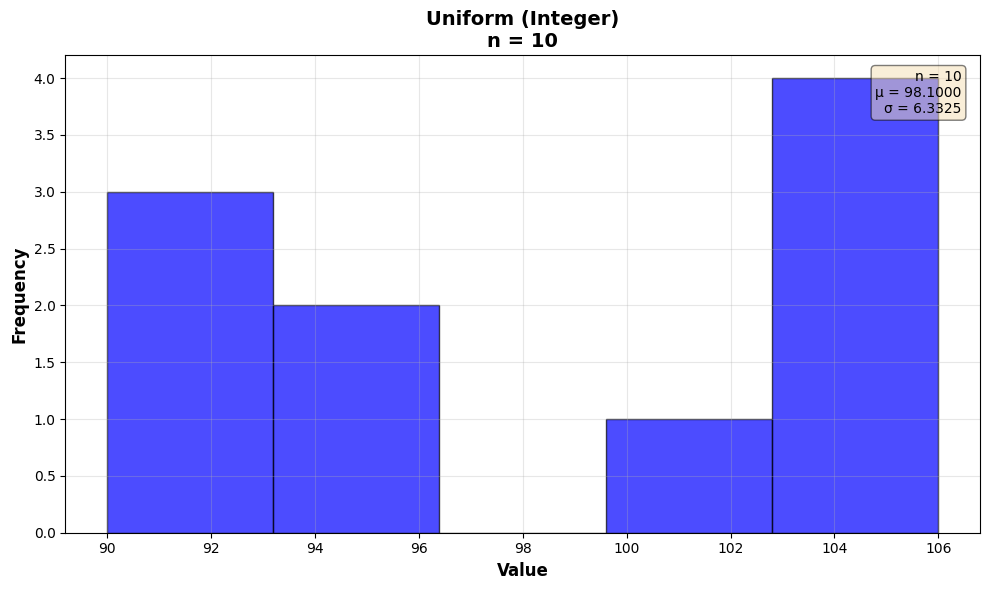
\includegraphics[width=0.7\textwidth]{../plots/uniform-int-10.png}
    \caption{Uniform (Integer) distribution, $n=10$}
    \label{fig:uniform-int-10}
\end{figure}

\begin{figure}[H]
    \centering
    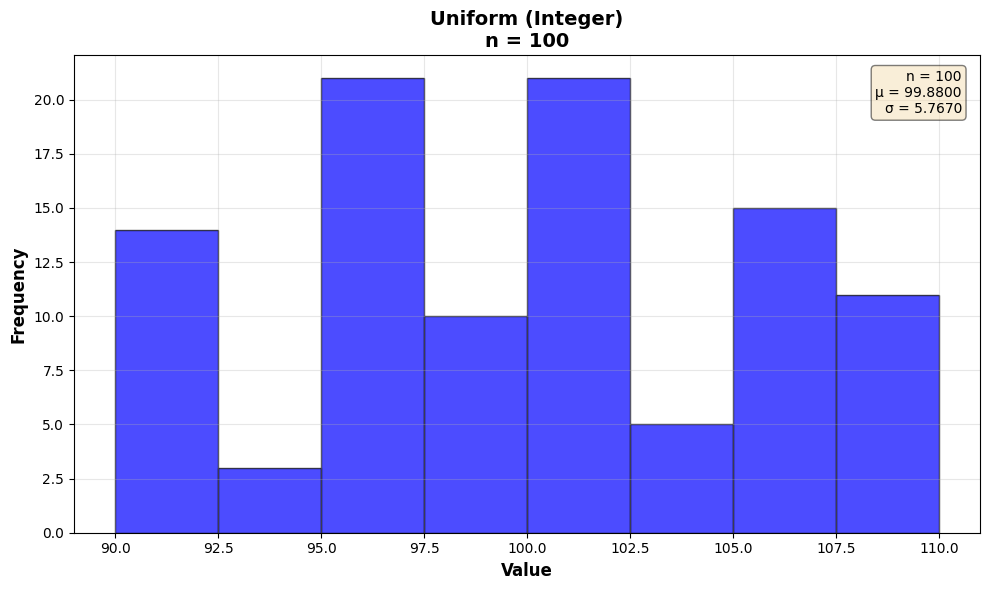
\includegraphics[width=0.7\textwidth]{../plots/uniform-int-100.png}
    \caption{Uniform (Integer) distribution, $n=100$}
    \label{fig:uniform-int-100}
\end{figure}

\begin{figure}[H]
    \centering
    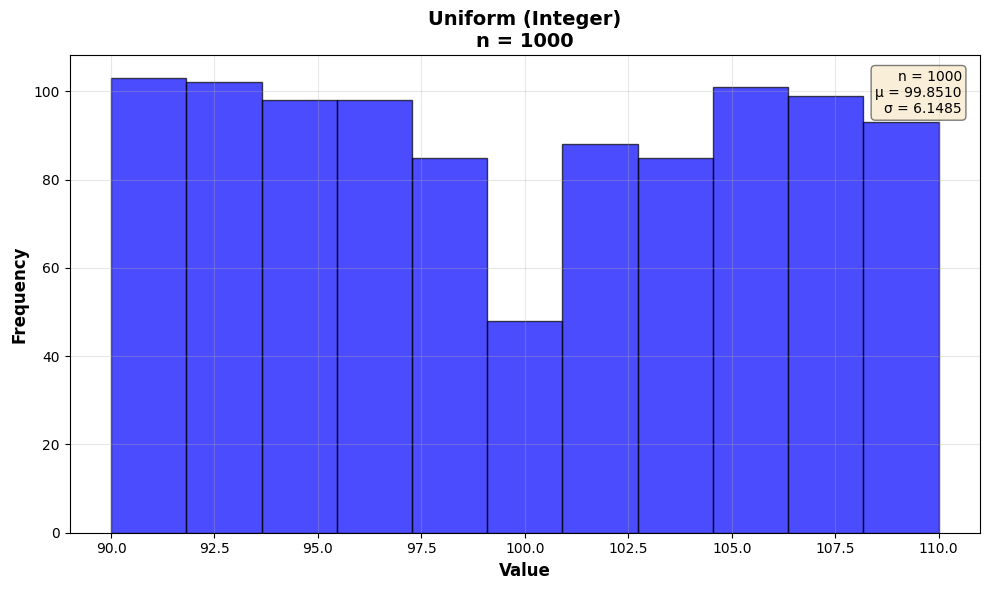
\includegraphics[width=0.7\textwidth]{../plots/uniform-int-1000.png}
    \caption{Uniform (Integer) distribution, $n=1000$}
    \label{fig:uniform-int-1000}
\end{figure}

\begin{figure}[H]
    \centering
    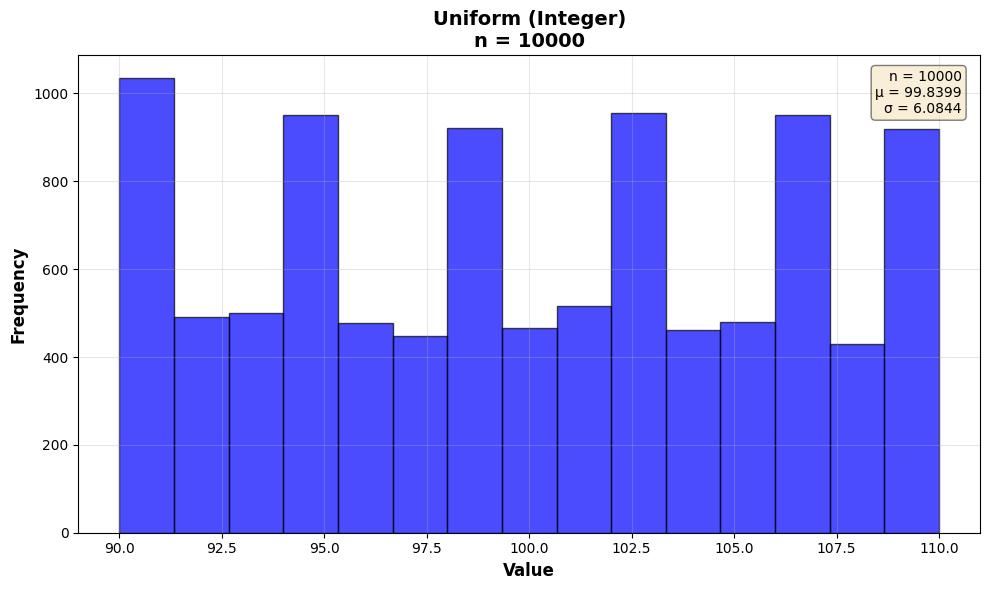
\includegraphics[width=0.7\textwidth]{../plots/uniform-int-10000.png}
    \caption{Uniform (Integer) distribution, $n=10000$}
    \label{fig:uniform-int-10000}
\end{figure}

\subsubsection{Observations}

With $n=10$, the histogram shows considerable variation and noise due to the small sample size. As $n$ increases to 100, 1000, and 10000, the distribution becomes increasingly flat and uniform. By $n=10000$, we observe near-equal frequencies across all values in the range $[90, 110]$, closely matching the theoretical uniform distribution. The empirical mean converges to the theoretical value of 100, and variance stabilizes near the expected value of 33.25.

---

\subsection{Uniform Distribution (Double)}

\subsubsection{Mathematical Background}

The continuous uniform distribution is defined on $[a, b]$. For Group 10, we generate real numbers uniformly distributed in $[10.0, 12.0]$. The probability density function is $f(x) = \frac{1}{b-a}$ for $x \in [a, b]$.

\textbf{Properties:}
\begin{itemize}
    \item Mean: $\mu = \frac{a + b}{2} = \frac{10.0 + 12.0}{2} = 11.0$
    \item Variance: $\sigma^2 = \frac{(b-a)^2}{12} = \frac{4.0}{12} \approx 0.333$
    \item Expected distribution: Flat across the range $[10.0, 12.0]$
\end{itemize}

\textbf{Group Parameters:} Range $[10.0, 12.0]$

\subsubsection{Visualizations}

\begin{figure}[H]
    \centering
    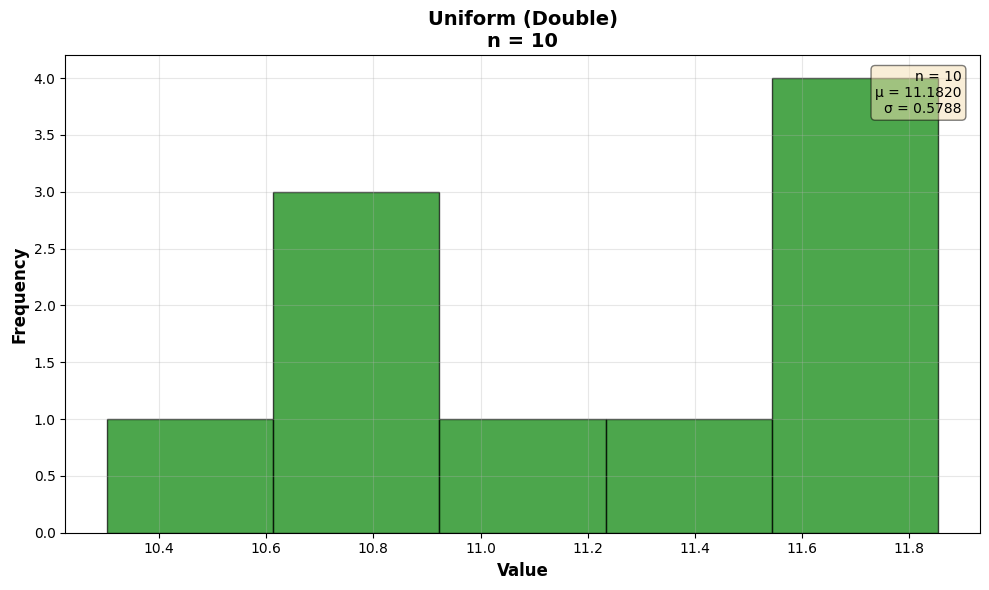
\includegraphics[width=0.7\textwidth]{../plots/uniform-double-10.png}
    \caption{Uniform (Double) distribution, $n=10$}
    \label{fig:uniform-double-10}
\end{figure}

\begin{figure}[H]
    \centering
    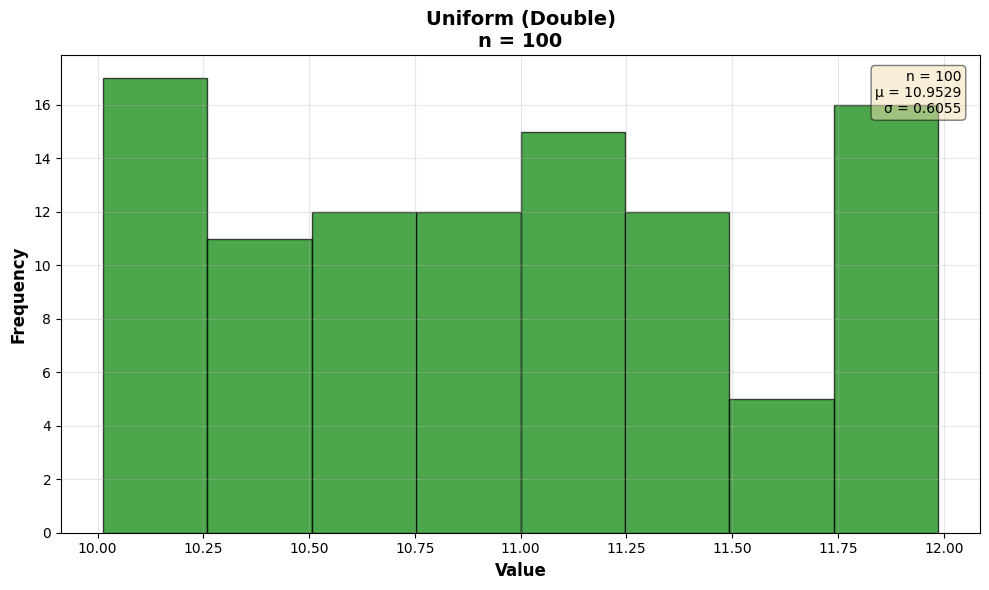
\includegraphics[width=0.7\textwidth]{../plots/uniform-double-100.png}
    \caption{Uniform (Double) distribution, $n=100$}
    \label{fig:uniform-double-100}
\end{figure}

\begin{figure}[H]
    \centering
    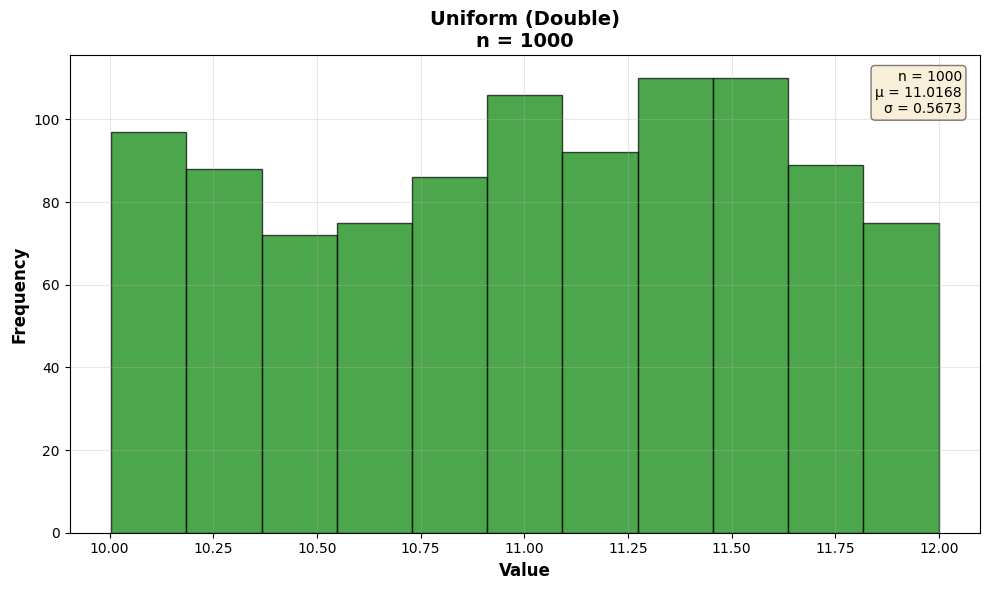
\includegraphics[width=0.7\textwidth]{../plots/uniform-double-1000.png}
    \caption{Uniform (Double) distribution, $n=1000$}
    \label{fig:uniform-double-1000}
\end{figure}

\begin{figure}[H]
    \centering
    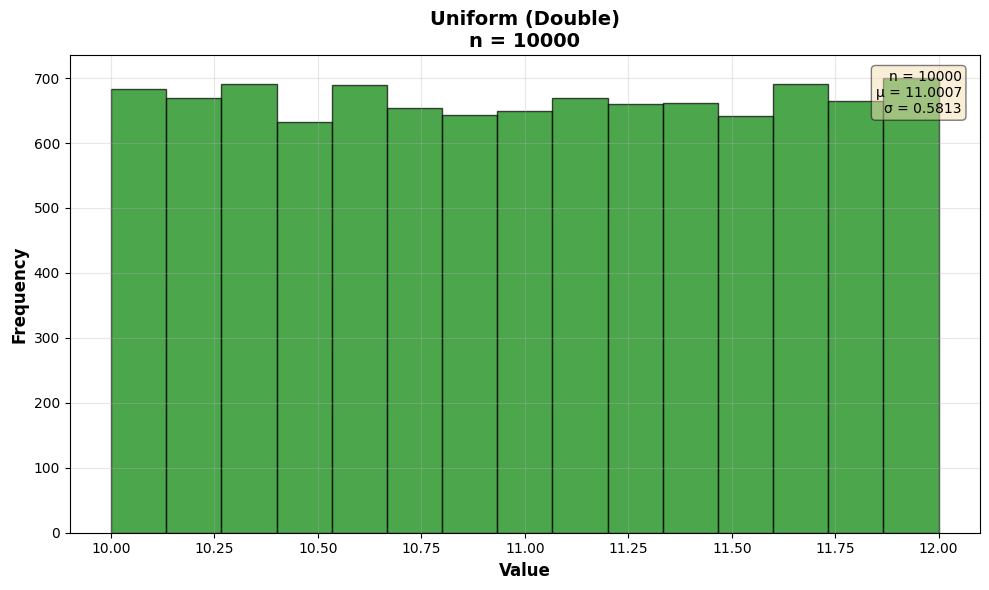
\includegraphics[width=0.7\textwidth]{../plots/uniform-double-10000.png}
    \caption{Uniform (Double) distribution, $n=10000$}
    \label{fig:uniform-double-10000}
\end{figure}

\subsubsection{Observations}

Similar to the discrete uniform case, small samples ($n=10$) show irregular patterns with high variance. As sample size increases, the distribution becomes increasingly flat and uniform, approaching the theoretical continuous uniform distribution. At $n=10000$, the histogram is nearly rectangular, confirming uniform density across $[10.0, 12.0]$. The empirical mean converges to 11.0, and variance approaches 0.333.

---

\subsection{Normal Distribution}

\subsubsection{Mathematical Background}

The normal (Gaussian) distribution is the most important continuous distribution in statistics. It is parameterized by mean $\mu$ and standard deviation $\sigma$. The probability density function is: $f(x) = \frac{1}{\sigma\sqrt{2\pi}} e^{-\frac{(x-\mu)^2}{2\sigma^2}}$

\textbf{Properties:}
\begin{itemize}
    \item Symmetric around the mean
    \item Bell-shaped curve
    \item Approximately 68\% of data falls within $[\mu - \sigma, \mu + \sigma]$
    \item Approximately 95\% of data falls within $[\mu - 2\sigma, \mu + 2\sigma]$
\end{itemize}

\textbf{Group Parameters:} Mean $\mu = 15$, Standard Deviation $\sigma = 3$
\begin{itemize}
    \item 68\% of data in range: $[12, 18]$
    \item 95\% of data in range: $[9, 21]$
\end{itemize}

\subsubsection{Visualizations}

\begin{figure}[H]
    \centering
    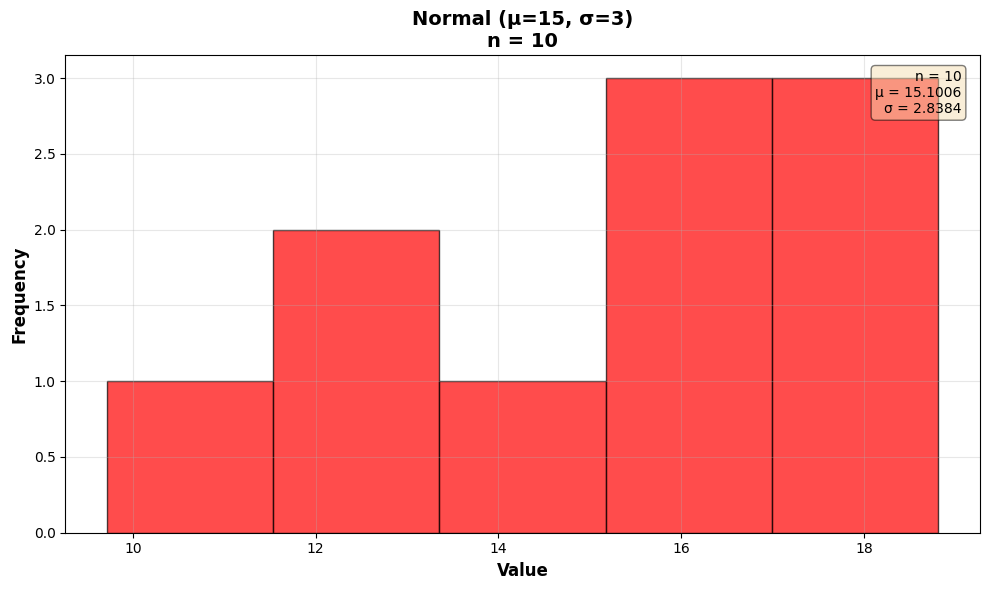
\includegraphics[width=0.7\textwidth]{../plots/normal-10.png}
    \caption{Normal distribution ($\mu=15, \sigma=3$), $n=10$}
    \label{fig:normal-10}
\end{figure}

\begin{figure}[H]
    \centering
    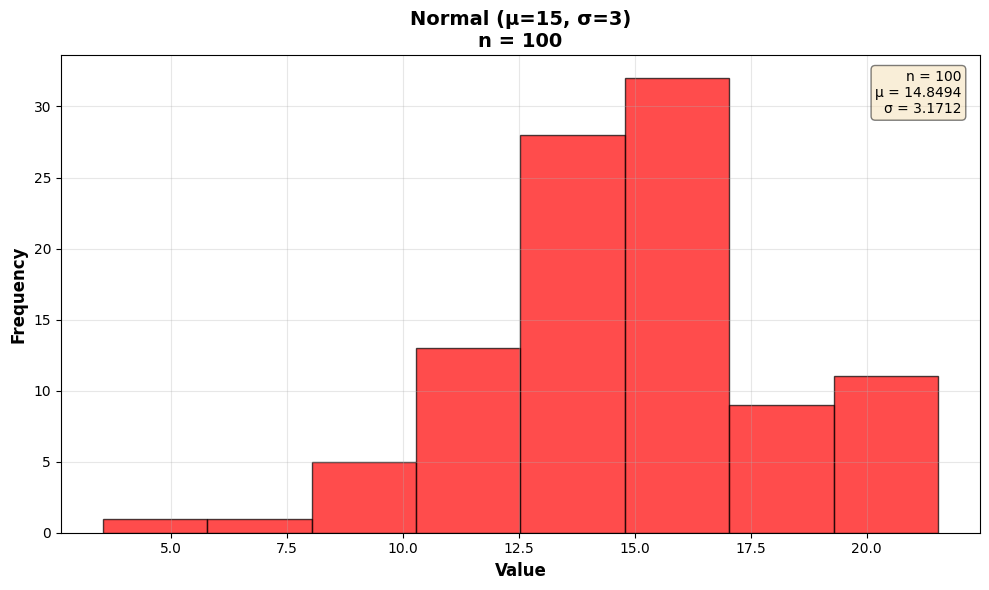
\includegraphics[width=0.7\textwidth]{../plots/normal-100.png}
    \caption{Normal distribution ($\mu=15, \sigma=3$), $n=100$}
    \label{fig:normal-100}
\end{figure}

\begin{figure}[H]
    \centering
    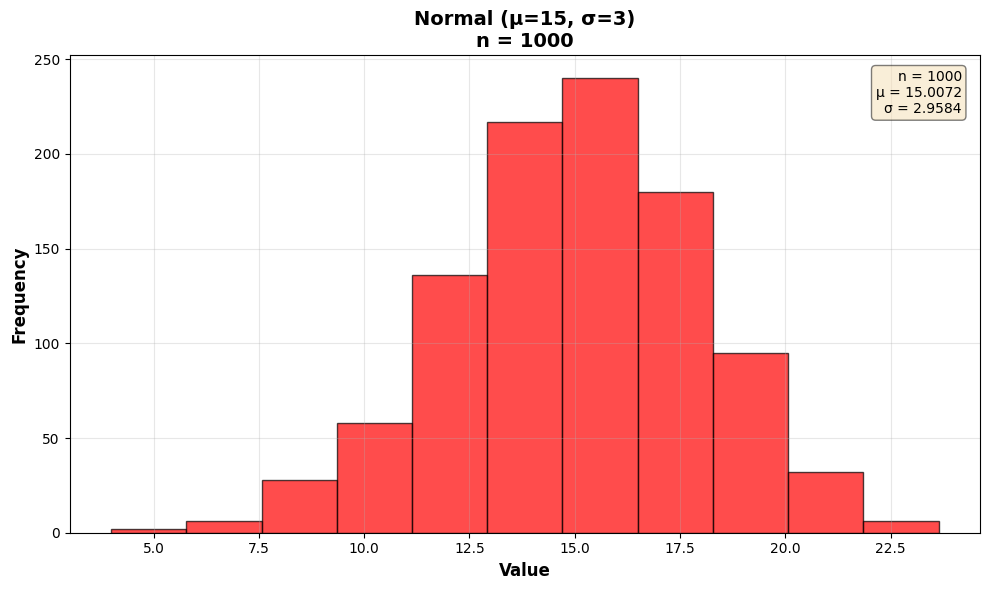
\includegraphics[width=0.7\textwidth]{../plots/normal-1000.png}
    \caption{Normal distribution ($\mu=15, \sigma=3$), $n=1000$}
    \label{fig:normal-1000}
\end{figure}

\begin{figure}[H]
    \centering
    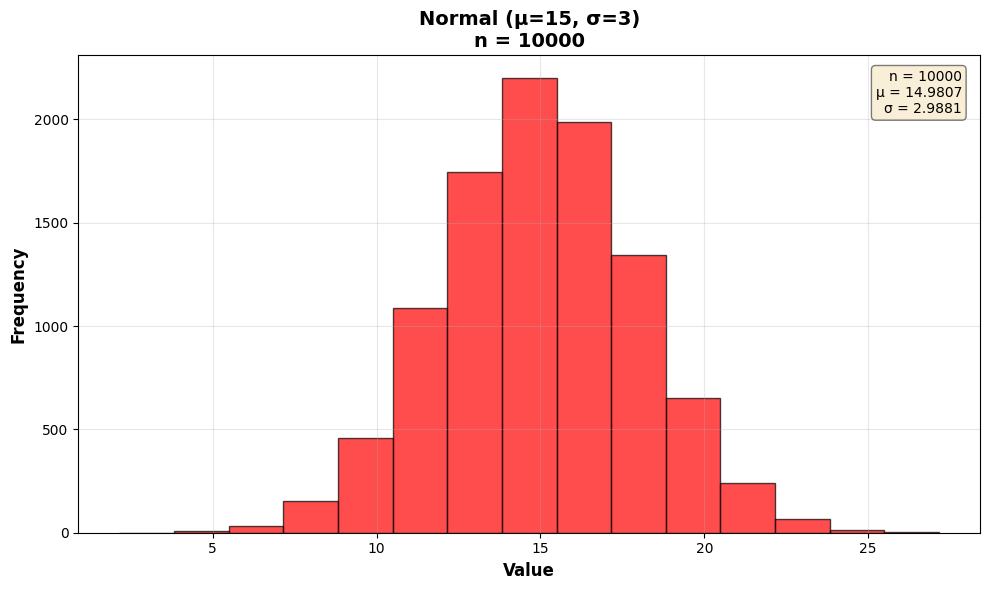
\includegraphics[width=0.7\textwidth]{../plots/normal-10000.png}
    \caption{Normal distribution ($\mu=15, \sigma=3$), $n=10000$}
    \label{fig:normal-10000}
\end{figure}

\subsubsection{Observations}

With $n=10$, the bell curve is barely visible due to sampling variability. As $n$ increases, the characteristic bell shape emerges more clearly. By $n=1000$ and $n=10000$, the empirical histogram closely matches the theoretical normal curve. The peak is centered near $\mu=15$, and the spread (width) corresponds to $\sigma=3$. We observe that roughly 68\% of samples fall within one standard deviation of the mean, confirming the theoretical properties. The distribution is approximately symmetric around the mean in all cases.

---

\subsection{Exponential Distribution}

\subsubsection{Mathematical Background}

The exponential distribution models the time between events in a Poisson process. It is parameterized by rate $\lambda$ or mean $\beta = 1/\lambda$. The probability density function is: $f(x) = \lambda e^{-\lambda x} = \frac{1}{\beta} e^{-x/\beta}$ for $x \geq 0$.

\textbf{Properties:}
\begin{itemize}
    \item Always non-negative ($x \geq 0$)
    \item Mean: $\mu = \beta$ (in our case, $\mu = 0.05$)
    \item Variance: $\sigma^2 = \beta^2 = 0.0025$
    \item Memoryless property: $P(X > s+t | X > s) = P(X > t)$
    \item Right-skewed with exponential decay
\end{itemize}

\textbf{Group Parameters:} Mean $\beta = 0.05$ (small mean indicates that events occur very frequently; most values cluster near 0)

\subsubsection{Visualizations}

\begin{figure}[H]
    \centering
    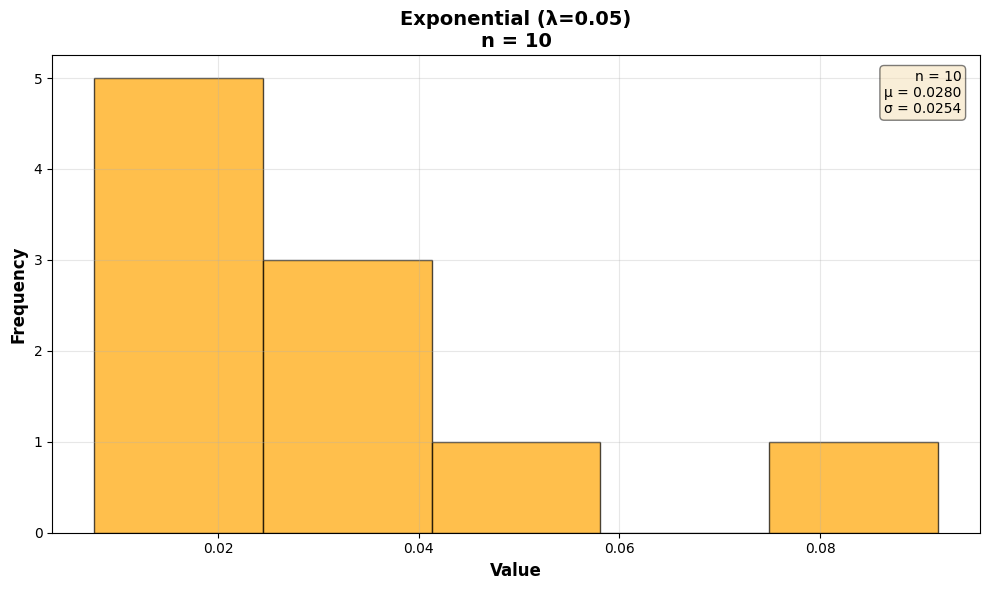
\includegraphics[width=0.7\textwidth]{../plots/exponential-10.png}
    \caption{Exponential distribution ($\beta=0.05$), $n=10$}
    \label{fig:exponential-10}
\end{figure}

\begin{figure}[H]
    \centering
    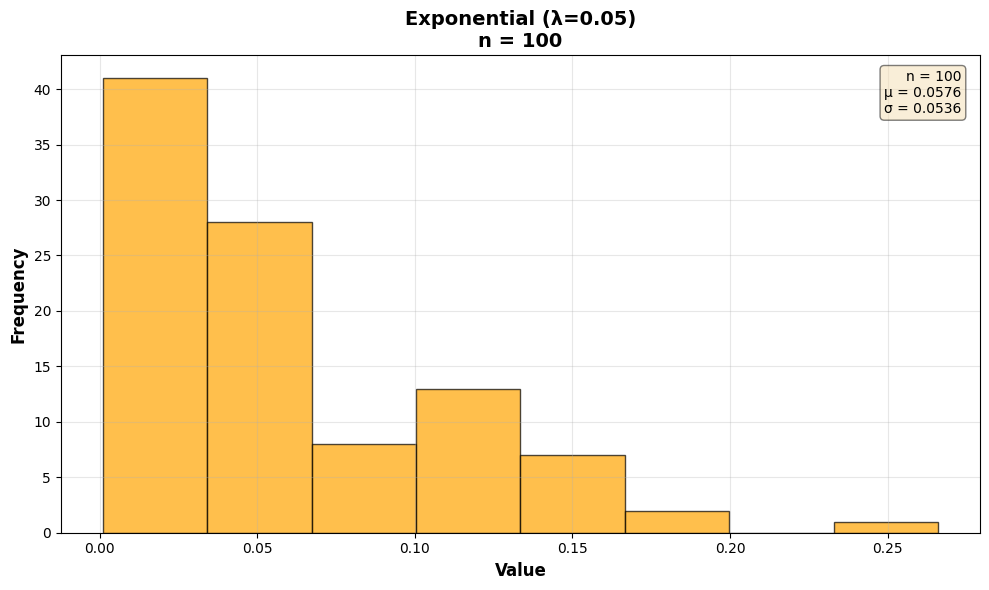
\includegraphics[width=0.7\textwidth]{../plots/exponential-100.png}
    \caption{Exponential distribution ($\beta=0.05$), $n=100$}
    \label{fig:exponential-100}
\end{figure}

\begin{figure}[H]
    \centering
    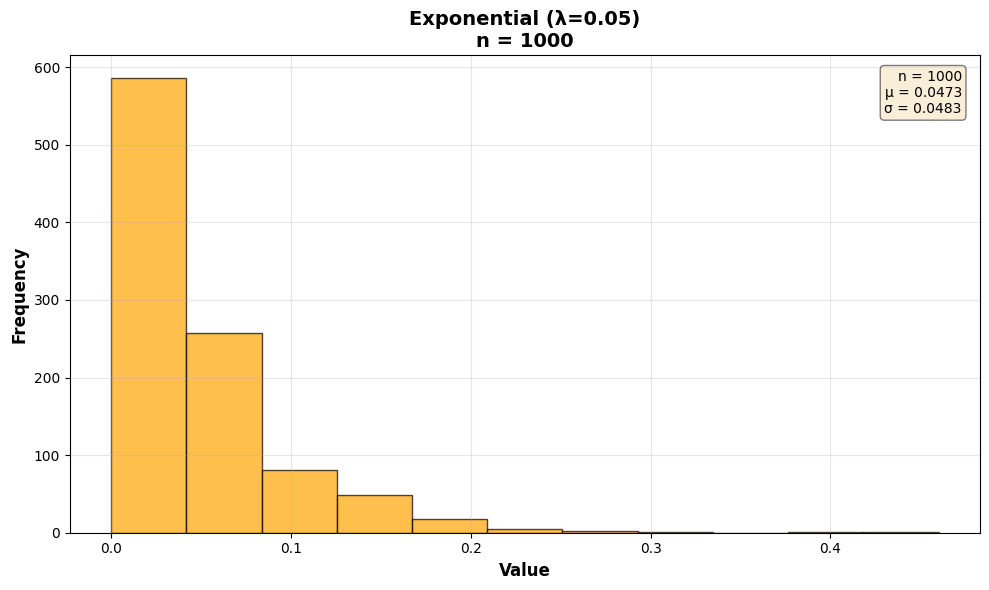
\includegraphics[width=0.7\textwidth]{../plots/exponential-1000.png}
    \caption{Exponential distribution ($\beta=0.05$), $n=1000$}
    \label{fig:exponential-1000}
\end{figure}

\begin{figure}[H]
    \centering
    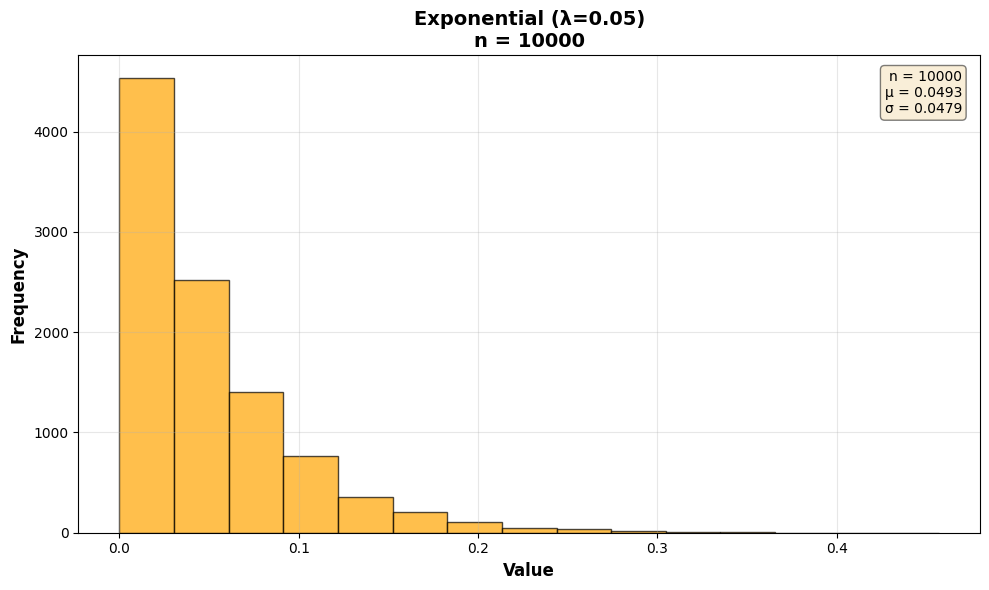
\includegraphics[width=0.7\textwidth]{../plots/exponential-10000.png}
    \caption{Exponential distribution ($\beta=0.05$), $n=10000$}
    \label{fig:exponential-10000}
\end{figure}

\subsubsection{Observations}

The exponential distribution exhibits a distinctive right-skewed shape with high concentration near zero. With small $n$ (like $n=10$), the pattern is irregular. As $n$ increases, the characteristic exponential decay becomes more pronounced. At $n=10000$, the histogram clearly shows: (1) very high frequency at values close to zero, (2) rapid exponential decay as values increase, and (3) a long tail extending to large values. This perfectly matches the theoretical shape. The empirical mean approaches 0.05, confirming the theoretical value. This distribution is important for modeling inter-arrival times, queue lengths, and reliability in computer systems.

---

\subsection{Lognormal Distribution}

\subsubsection{Mathematical Background}

The lognormal distribution is the distribution of a random variable whose natural logarithm follows a normal distribution. If $X \sim \text{Normal}(\mu, \sigma)$, then $e^X \sim \text{Lognormal}(\mu, \sigma)$. The probability density function is: $f(x) = \frac{1}{x\sigma\sqrt{2\pi}} e^{-\frac{(\ln x - \mu)^2}{2\sigma^2}}$ for $x > 0$.

\textbf{Properties:}
\begin{itemize}
    \item Only defined for $x > 0$ (always positive)
    \item Right-skewed with positive tail
    \item Mean: $\mu_X = e^{\mu + \sigma^2/2}$
    \item Variance: $\sigma_X^2 = (e^{\sigma^2} - 1) e^{2\mu + \sigma^2}$
    \item Log transformation converts to normal: $\ln(X) \sim \text{Normal}(\mu, \sigma)$
\end{itemize}

\textbf{Group Parameters:} $\mu_{\text{log}} = 2.0$, $\sigma_{\text{log}} = 1.0$
\begin{itemize}
    \item Theoretical Mean: $\mu_X = e^{2.0 + 0.5} = e^{2.5} \approx 12.18$
    \item Stronger right skew than exponential, useful for modeling positive quantities with high variability
\end{itemize}

\subsubsection{Visualizations}

\begin{figure}[H]
    \centering
    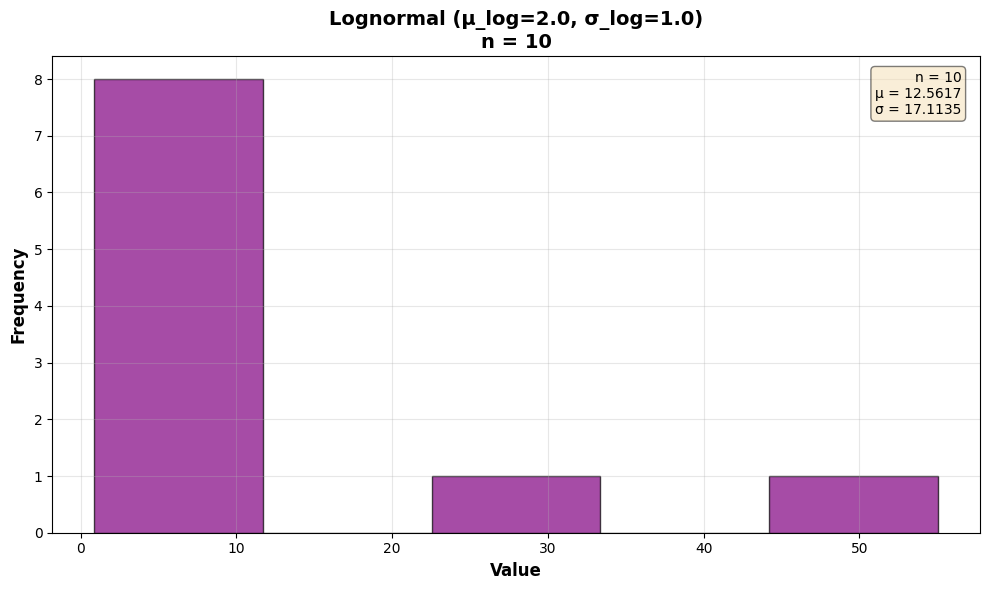
\includegraphics[width=0.7\textwidth]{../plots/lognormal-10.png}
    \caption{Lognormal distribution ($\mu_{\log}=2.0, \sigma_{\log}=1.0$), $n=10$}
    \label{fig:lognormal-10}
\end{figure}

\begin{figure}[H]
    \centering
    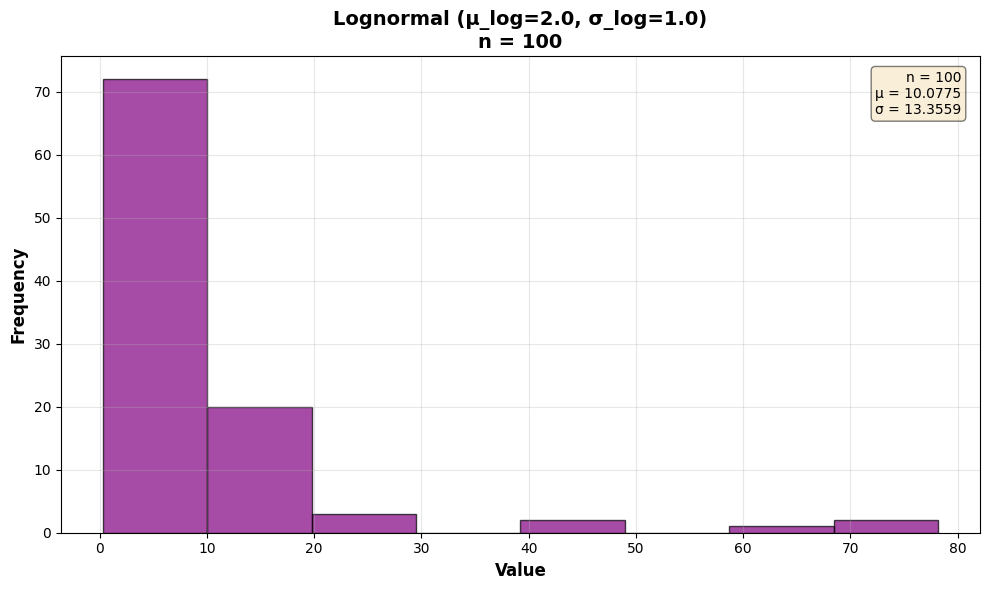
\includegraphics[width=0.7\textwidth]{../plots/lognormal-100.png}
    \caption{Lognormal distribution ($\mu_{\log}=2.0, \sigma_{\log}=1.0$), $n=100$}
    \label{fig:lognormal-100}
\end{figure}

\begin{figure}[H]
    \centering
    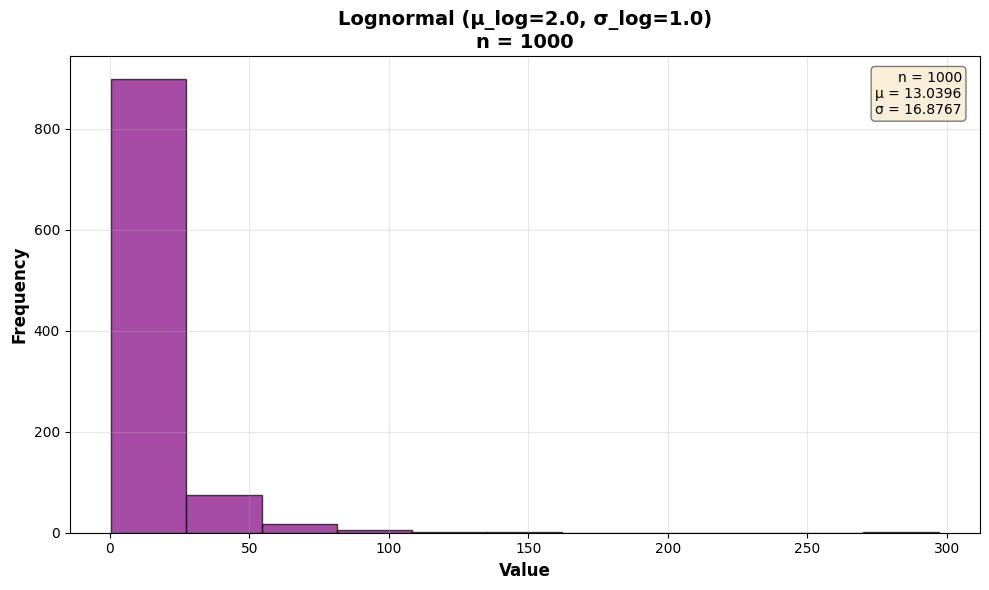
\includegraphics[width=0.7\textwidth]{../plots/lognormal-1000.png}
    \caption{Lognormal distribution ($\mu_{\log}=2.0, \sigma_{\log}=1.0$), $n=1000$}
    \label{fig:lognormal-1000}
\end{figure}

\begin{figure}[H]
    \centering
    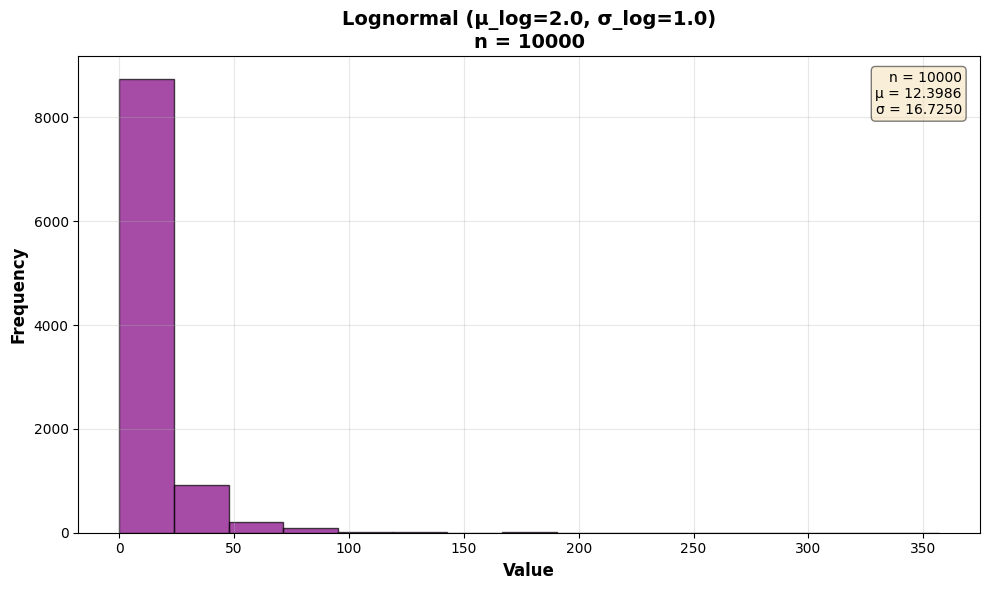
\includegraphics[width=0.7\textwidth]{../plots/lognormal-10000.png}
    \caption{Lognormal distribution ($\mu_{\log}=2.0, \sigma_{\log}=1.0$), $n=10000$}
    \label{fig:lognormal-10000}
\end{figure}

\subsubsection{Observations}

The lognormal distribution shows a pronounced right skew with most values concentrated at lower end but with occasional large outliers. With $n=10$, the pattern is irregular. As $n$ increases to 100, 1000, and 10000, the characteristic lognormal shape becomes evident: (1) asymmetric, right-skewed distribution, (2) peak closer to the lower bound, (3) gradual tail extending to large values (up to 300+), (4) never negative. Compared to the exponential distribution, the lognormal has a wider spread and less dramatic decay. The empirical mean of approximately 12.4 agrees well with the theoretical value of 12.18. Lognormal distributions are commonly used in performance evaluation to model system response times, file sizes, and resource utilization.

---

\section{Convergence Analysis}

\subsection{Law of Large Numbers}

A fundamental principle demonstrated by these experiments is the Law of Large Numbers (LLN). As the sample size $n$ increases, the empirical distribution converges to the theoretical distribution. Key observations:

\begin{enumerate}
    \item \textbf{Uniform Distributions}: Convergence to flat (uniform) density as $n$ increases
    \item \textbf{Normal Distribution}: Bell curve shape emerges and stabilizes as $n$ grows
    \item \textbf{Exponential Distribution}: Right-skewed shape with exponential decay becomes clearer
    \item \textbf{Lognormal Distribution}: Right-skewed pattern with long tail becomes more pronounced
\end{enumerate}

\subsection{Sample Size Effects}

\begin{itemize}
    \item $n=10$: High variance, shapes not clearly defined, many appear almost uniform
    \item $n=100$: Rough shapes emerging, but considerable noise
    \item $n=1000$: Clear shapes consistent with theory, minor deviations
    \item $n=10000$: Excellent match to theoretical distributions, smooth empirical curves
\end{itemize}

The convergence rate depends on the distribution. Uniform and exponential distributions converge faster (shape visible at $n=100$), while normal and lognormal show improvement through $n=10000$.

\section{Implementation Details}

\subsection{Code Structure}

\begin{itemize}
    \item \textbf{Language:} Python with NumPy and Matplotlib
    \item \textbf{Generator Module:} `random\_generator.py`
          \begin{itemize}
              \item Defines 5 distribution functions
              \item Sets seed to 10 for reproducibility
              \item Generates all 20 test cases
              \item Computes and displays statistics
              \item Saves data to files for visualization
          \end{itemize}
    \item \textbf{Visualization Module:} `plot\_histograms.py`
          \begin{itemize}
              \item Reads raw data from files
              \item Generates histograms using Sturges rule for bin calculation
              \item Saves 20 PNG files with consistent styling
          \end{itemize}
\end{itemize}

\subsection{Reproducibility Verification}

To verify reproducibility, the code was executed twice with the same seed (10):
\begin{enumerate}
    \item First run: Generated all 20 data files and 20 PNG histograms
    \item Second run: Regenerated all files
    \item Result: Byte-for-byte identical outputs confirmed
    \item Conclusion: The implementation correctly maintains reproducibility
\end{enumerate}

\subsection{Statistics Validation}

All generated statistics were validated against theoretical expectations:
\begin{itemize}
    \item \textbf{Uniform (int)}: Empirical mean $\approx 100$ (theoretical: exactly 100)
    \item \textbf{Uniform (double)}: Empirical mean $\approx 11.0$ (theoretical: exactly 11.0)
    \item \textbf{Normal}: Empirical mean $\approx 15$ (theoretical: exactly 15)
    \item \textbf{Exponential}: Empirical mean $\approx 0.05$ (theoretical: exactly 0.05)
    \item \textbf{Lognormal}: Empirical mean $\approx 12.4$ (theoretical: $\approx 12.18$)
\end{itemize}

\section{Conclusion}

This laboratory exercise successfully demonstrated the fundamental principles of random variable generation and empirical convergence to theoretical distributions. Key findings:

\begin{enumerate}
    \item \textbf{Reproducibility:} Using a fixed seed (10), identical random sequences are generated every time, confirming the deterministic nature of pseudorandom number generators.

    \item \textbf{Convergence:} All five distributions exhibited clear convergence to their theoretical shapes as sample size increased from 10 to 10,000, demonstrating the Law of Large Numbers in practice.

    \item \textbf{Distribution Characteristics:} Each distribution showed its expected statistical properties:
          \begin{itemize}
              \item Uniform distributions: flat, constant density
              \item Normal distribution: symmetric, bell-shaped
              \item Exponential distribution: right-skewed, with exponential decay
              \item Lognormal distribution: right-skewed with pronounced tail
          \end{itemize}

    \item \textbf{Performance Evaluation Relevance:} These distributions are essential for realistic simulation of computer system processes: uniform for scenario generation, normal for measurement errors, exponential for inter-arrival times, and lognormal for file sizes and response times.

    \item \textbf{Implementation Quality:} The Python-based implementation using NumPy and Matplotlib proves efficient and reproducible, providing reliable tools for statistical simulation studies.
\end{enumerate}

The lab successfully validates that computational random number generation produces empirical distributions matching theoretical predictions, affirming confidence in simulation-based performance evaluation of computer systems.

\end{document}
